% !TEX root=../MA119-Main.tex


\paragraph*{The Graph of a Quadratic Function}
	The graph of a quadratic function $f(x)=ax^2+bx+c$, $a\neq 0$, is called a parabola.

	A quadratic function $f(x)=ax^2+bx+c$ can be written in the form $f(x)=a(x-h)^2+k$, where $h=-\dfrac{b}{2a}$ and $k=f(h)=f\left(-\dfrac{b}{2a}\right)$.
	\begin{itemize}
		\item  The line $x=h=-\dfrac{b}{2a}$ is called the axis of symmetry of the parabola.
		\item The point $(h, k)=\left(-\dfrac{b}{2a}, f\left(-\dfrac{b}{2a}\right)\right)$ is called the vertex of the parabola.
	\end{itemize}

\paragraph*{The Minimum or Maximum of a Quadratic Function}
	Consider the quadratic function $f(x)=ax^2+bx+c$, $a\neq 0$.

	\begin{itemize}
		\item If $a>0$, then the parabola opens upward and $f$ has a minimum  $f\left(-\dfrac{b}{2a}\right)$ at the vertex.
		\item If $a<0$, then the parabola opens downward and $f$ has a maximum  $f\left(-\dfrac{b}{2a}\right)$ at the vertex.
	\end{itemize}

\paragraph*{Intercepts of a Quadratic Function}
	Consider the quadratic function $f(x)=ax^2+bx+c$, $a\neq 0$.
	\begin{itemize}
		\item The $y$-intercept is $(0, f(0))=(0, c)$.
		\item  The $x$-intercepts, if exist, are the solutions of the equation $ax^2+bx+c=0$.
	\end{itemize}

	\begin{example}
		Does the function $f(x)=2x^2-4x-6$ have a maximum or minimum? Find it.
	\end{example}

	\begin{solution}\mbox{}\vspace{-0.25em}
		\begin{enumerate}[label={\textbf{\textup{Step \arabic*.}}~}]
			\item Since $a>2$, the function opens upward and has a minimum.
			\item Find the line of symmetry $x=\frac{-b}{2a}$:
			      $x=\frac{-(-4)}{2\cdot 2}=1$.
			\item Find the minimum by plugging $x=1$ into the function $f$.
				  The minimum is
				  $$
				  f(-\frac{b}{2a})=f(1)=2-4-6=-8.
				  $$
		\end{enumerate}
	\end{solution}

	\begin{example}
		Consider the function $f(x)=-x^2+3x+6$. Find values of $x$ such that $f(x)=2$.
	\end{example}
	\begin{solution}\mbox{}\vspace{-0.25em}
		\begin{enumerate}[label={\textbf{\textup{Step \arabic*.}}~}]
			\item Set up the equation for $x$.
			      \[-x^2+3x+6=2\]
			\item Solve the equation $-x^2+3x+6=2$.

			      We get $x=-1$ or $x=4$.
			      % \[\begin{split}
			      % -x^2+3x+6&=2\\
			      % -x^2+3x+4&=0\\
			      % x^2-3x-4&=0\\
			      % (x+1)(x-4)&=0
			      % \end{split}\]
			      % \begin{alignat*}{3}
			      % 	x&=-1 && \ctc{or} & x&=4
			      % \end{alignat*}
		\end{enumerate}
		The values of $x$ such that $f(x)=2$ are $x=-1$ and $x=44$.
	\end{solution}

	\begin{example}
		A quadratic function $f$ whose the vertex is $(1, 2)$ has a $y$-intercept $(0, -3)$. Find the equation that defines the function.
	\end{example}
	\begin{solution}\mbox{}\vspace{-0.25em}
		\begin{enumerate}[label={\textbf{\textup{Step \arabic*.}}~}]
			\item Write down the general form of $f$ using only the vertex.

			      Quadratic functions with the vertex at $(1,2)$ are defined by $y=a(x-1)^2+2$, where $a$ is a nonzero real number.
			\item Determine the unknown $a$ using the remaining information.

			      Since $(0, -3)$ is on the graph of the function, the number $a$ must satisfy the equation  $-3=a(0-1)^2+2$.
			\item
			      Solving for $a$ from the equation, we get $a=-5$.

			      The quadratic function $f$ is given by $f(x)=-5(x-1)^2+2$.
		\end{enumerate}
	\end{solution}





\newpage

\begin{exercise}
	Sketch the graph of the quadratic functions $f(x)=-(x-2)^2+4$ and find
	
\begin{multicols}{2}
	\begin{enumerate}[label={(\arabic*)~ }]
		\item
			  the coordinates of the $x$-intercepts,
		\item the coordinates of the $y$-intercept,
		\item the equation of the axis of symmetry,
		\item the coordinates of the vertex.
		\item the interval of $x$ values such that $f(x)\geq 0$.
		\end{enumerate}

\columnbreak

	\begin{center}
		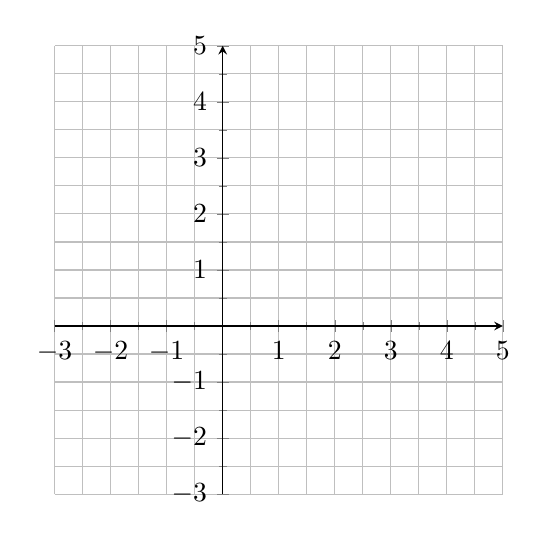
\begin{tikzpicture}[scale=1]
			\begin{axis}[grid=both, unit vector ratio*=1 1, ymin=-3,ymax=5,xmax=5,xmin=-3,xtick={-4,-3,...,5},ytick={-3,-2,...,5},minor tick num=1, axis lines = middle
				]
				%\addplot[thick, samples=100,domain=1:3.82, name path=A, -stealth]   {(x-2)^2+1};
				% \addplot[thick, draw] (1, 2)--(-1.95,1.5);
				% \node[draw,shape=circle, minimum size=1.25mm,inner sep=0pt,outer sep=0pt] at (-2,1.5) {};
			\end{axis}
		\end{tikzpicture}
	\end{center}
\end{multicols}
\end{exercise}

\vfill
\begin{center} \hfill
	\raisebox{0.4em}{
		\rotatebox{\rotationdegree}{
			\parbox{\textwidth}{
				\begin{enumerate*}[label={\theexer~(\arabic*)~}]
					\item $(0,0)$ and $(4,0)$,
					\item $(0,0)$,
					\item $x=2$,
					\item $(2, 4)$,
					\item $[0, 4]$.
				\end{enumerate*}
			}
		}
	}
\end{center}

\begin{exercise}
	Sketch the graph of the quadratic functions $f(x)=x^2+2x-3$ and find
	
\begin{multicols}{2}
	\begin{enumerate}[label={(\arabic*)~ }]
		\item the coordinates of the $x$-intercepts,
		\item the coordinates of the $y$-intercept,
		\item the equation of the axis of symmetry,
		\item the coordinates of the vertex.
		\item the interval of $x$ values such that $f(x)>0$.
		\end{enumerate}

\columnbreak

	\begin{center}
		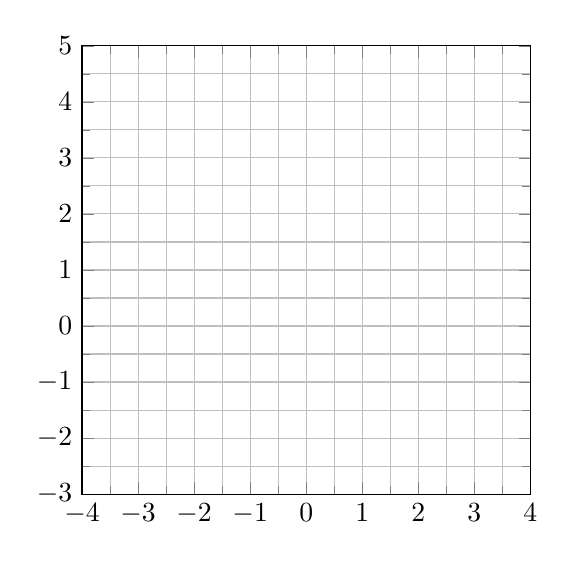
\begin{tikzpicture}[scale=1]
			\begin{axis}[grid=both, unit vector ratio*=1 1, ymin=-3,ymax=5,xmax=4,xmin=-4,xtick={-4,-3,...,4},ytick={-3,-2,...,5},minor tick num=1
				]
				%\addplot[thick, samples=100,domain=1:3.82, name path=A, -stealth]   {(x-2)^2+1};
				% \addplot[thick, draw] (1, 2)--(-1.95,1.5);
				% \node[draw,shape=circle, minimum size=1.25mm,inner sep=0pt,outer sep=0pt] at (-2,1.5) {};
			\end{axis}
		\end{tikzpicture}
	\end{center}
\end{multicols}
\end{exercise}

\vfill
\begin{center} \hfill
	\raisebox{0.4em}{
		\rotatebox{\rotationdegree}{
			\parbox{\textwidth}{
				\begin{enumerate*}[label={\theexer~(\arabic*)~}]
					\item $(-3,0)$ and $(1,0)$,
					\item $(0,-3)$,
					\item $x=-1$,
					\item $(-1, -4)$,
					\item $(-\infty, -3)\cup (1, \infty)$.
				\end{enumerate*}
			}
		}
	}
\end{center}

\newpage


\begin{exercise}
	Consider the parabola in the graph.
	\begin{multicols}{2}
		\begin{enumerate}[label={(\arabic*)~}]
			% \item For what values of $x$ is $y$ negative? Express your answer in interval notation.
			% \item Find the domain of the function.
			% \item Find the range of the function.
			      % \item Determine the value of $f(0)$.
			\item Determine the coordinates of the $x$-intercepts.
			\item Determine the coordinates of the $y$-intercept.
			\item Determine the coordinates of the vertex.
			\item For what values of $x$ is $f(x)=-3$.
			\item Find an equation for the function. \vspace{0.5in}
		\end{enumerate}
		\columnbreak
		\begin{center}
			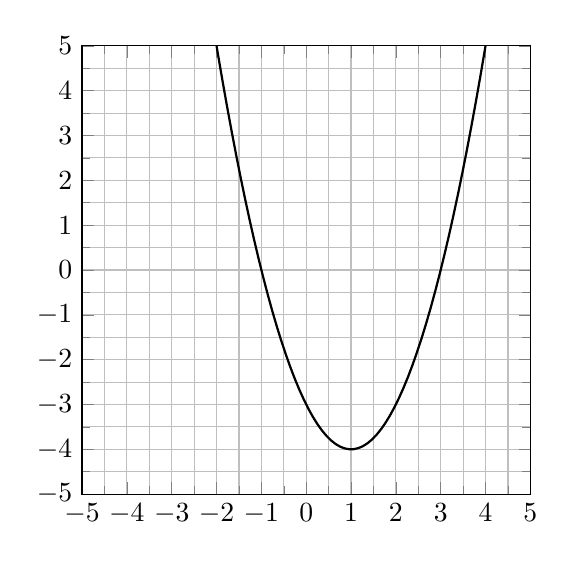
\begin{tikzpicture}[scale=1]
				\begin{axis}[grid=both,unit vector ratio*=1 1, ymin=-5,ymax=5,xmax=5,xmin=-5,xtick={-5,-4,...,5},ytick={-5,-4,...,5}, minor tick num=1
					]
					\addplot[thick, samples=100]   {(x-1)^2-4};
				\end{axis}
			\end{tikzpicture}
		\end{center}


	\end{multicols}
\end{exercise}

\vfill
\begin{center} \hfill
	\raisebox{0.4em}{
		\rotatebox{\rotationdegree}{
			\parbox{\textwidth}{
				\begin{enumerate*}[label={\theexer~(\arabic*)~}]
					% \item $(-1,3)$,
					% \item $(-\infty,\infty)$,
					% \item $[-4, \infty)$,
					\item $(-1, 0)$ and $(3, 0)$,
					\item $(0, -3)$,
					\item $(1,-4)$
					\item $x=0$ or $x=2$
					\item $f(x)=(x+1)(x-3)$\hfill\null
				\end{enumerate*}
			}
		}
	}
\end{center}

\begin{exercise}
	Consider the parabola in the graph.

	\begin{multicols}{2}
		\begin{enumerate}[label={(\arabic*)~}]
			% \item For what values of $x$ is $y$ negative? Express your answer in interval notation.
			% \item Find the domain of the function.
			% \item Find the range of the function.
			      % \item Determine the value of $f(0)$.
			\item Determine the coordinates of the $x$-intercepts.
			\item Determine the coordinates of the $y$-intercept.
			\item Determine the coordinates of the vertex.
			\item For what values of $x$ is $f(x)=\frac{3}{2}$.
			\item Find an equation for the function.
		\end{enumerate}
		\columnbreak
		\begin{center}
			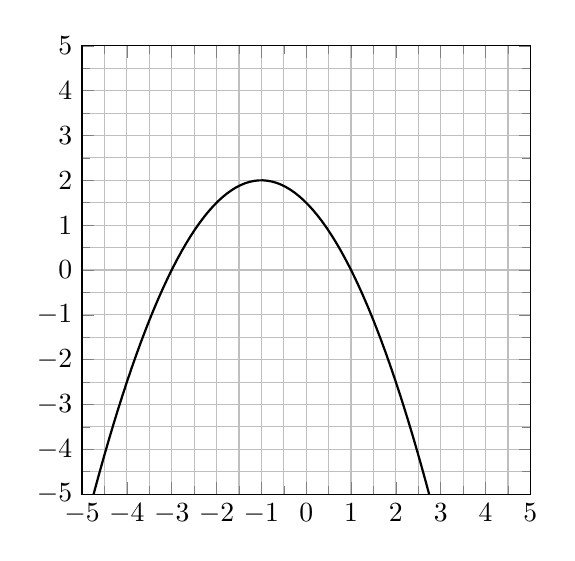
\begin{tikzpicture}[scale=1]
				\begin{axis}[grid=both,unit vector ratio*=1 1, ymin=-5,ymax=5,xmax=5,xmin=-5,xtick={-5,-4,...,5},ytick={-5,-4,...,5}, minor tick num=1
					]
					\addplot[thick, samples=100]   {(-(x+1)^2+4)/2};
				\end{axis}
			\end{tikzpicture}
		\end{center}
	\end{multicols}
\end{exercise}

\vfill
\begin{center} \hfill
	\raisebox{0.4em}{
		\rotatebox{\rotationdegree}{
			\parbox{\textwidth}{
				\begin{enumerate*}[label={\theexer~(\arabic*)~}]
					% \item $(-\infty,3)\cup (1, \infty)$,
					% \item $(-\infty,\infty)$,
					% \item $(-\infty, 2]$,
					\item $(-3, 0)$ and $(1, 0)$,
					\item $(0, 3/2)$,
					\item $(-1,2)$
					\item $x=0$ or $x=-2$
					\item $f(x)=-\frac12(x-1)(x+3).$\hfill\null
				\end{enumerate*}
			}
		}
	}
\end{center}

\newpage

\begin{exercise}
	A store owner estimates that by charging $x$ dollars each for a certain cell phone case, he can sell $d(x)=40 - x$ phone cases each week. The revenue in dollars is $R(x)=xd(x)$ when the selling price of a computer is $x$, Find the selling price that will maximize revenue, and then find the amount of the maximum revenue.
\end{exercise}

%%%%%%
\vfill
\begin{center} \hfill
	\raisebox{0.4em}{
		\rotatebox{\rotationdegree}{
			\parbox{\textwidth}{
				\begin{enumerate*}[label={\theexer~}]
					\item When the selling price is \$20/each, the revenue reaches the maximum \$400.\hfill\null
				\end{enumerate*}
			}
		}
	}
\end{center}

\begin{exercise}
	A ball is thrown upward from the ground with an initial velocity $v_0$ ft/sec. The height $h(t)$ of the ball after $t$ seconds is $h(t)= -16t^2 + v_0t$. The ball hits the ground after 4 seconds.
	Find the maximum height and how long it will take the ball to reach the maximum height.
\end{exercise}

%%%%%%
\vfill
\begin{center} \hfill
	\raisebox{0.4em}{
		\rotatebox{\rotationdegree}{
			\parbox{\textwidth}{
				\begin{enumerate*}[label={\theexer~}]
					\item After 2 seconds the ball reaches its maximum hight 64 feet.\hfill\null
				\end{enumerate*}
			}
		}
	}
\end{center}

